\chapter{\IfLanguageName{dutch}{Stand van zaken}{State of the art}}%
\label{ch:stand-van-zaken}

% Tip: Begin elk hoofdstuk met een paragraaf inleiding die beschrijft hoe
% dit hoofdstuk past binnen het geheel van de bachelorproef. Geef in het
% bijzonder aan wat de link is met het vorige en volgende hoofdstuk.

% Pas na deze inleidende paragraaf komt de eerste sectiehoofding.

% Dit hoofdstuk bevat je literatuurstudie. De inhoud gaat verder op de inleiding, maar zal het onderwerp van de bachelorproef *diepgaand* uitspitten. De bedoeling is dat de lezer na lezing van dit hoofdstuk helemaal op de hoogte is van de huidige stand van zaken (state-of-the-art) in het onderzoeksdomein. Iemand die niet vertrouwd is met het onderwerp, weet nu voldoende om de rest van het verhaal te kunnen volgen, zonder dat die er nog andere informatie moet over opzoeken \autocite{Pollefliet2011}.

% Je verwijst bij elke bewering die je doet, vakterm die je introduceert, enz.\ naar je bronnen. In \LaTeX{} kan dat met het commando \texttt{$\backslash${textcite\{\}}} of \texttt{$\backslash${autocite\{\}}}. Als argument van het commando geef je de ``sleutel'' van een ``record'' in een bibliografische databank in het Bib\LaTeX{}-formaat (een tekstbestand). Als je expliciet naar de auteur verwijst in de zin (narratieve referentie), gebruik je \texttt{$\backslash${}textcite\{\}}. Soms is de auteursnaam niet expliciet een onderdeel van de zin, dan gebruik je \texttt{$\backslash${}autocite\{\}} (referentie tussen haakjes). Dit gebruik je bv.~bij een citaat, of om in het bijschrift van een overgenomen afbeelding, broncode, tabel, enz. te verwijzen naar de bron. In de volgende paragraaf een voorbeeld van elk.

% \textcite{Knuth1998} schreef een van de standaardwerken over sorteer- en zoekalgoritmen. Experten zijn het erover eens dat cloud computing een interessante opportuniteit vormen, zowel voor gebruikers als voor dienstverleners op vlak van informatietechnologie~\autocite{Creeger2009}.

% Let er ook op: het \texttt{cite}-commando voor de punt, dus binnen de zin. Je verwijst meteen naar een bron in de eerste zin die erop gebaseerd is, dus niet pas op het einde van een paragraaf.

In de state of the art zullen we een beeld schetsen over de technologieën die
we toepassen in de ontwikkeling van onze webapplicatie. Daarnaast zal er een
vergelijking worden gemaakt op basis van kost, populariteit, leercurve,
prestaties, schaalbaarheid en ondersteuning.

Een framework is een set van tools gebruikt als basis om goed gestructureerde
en betrouwbare software en systemen te ontwikkelen. Een web development
framework wordt vaak gebruikt bij het ontwikkelen van een web applicatie.
Inclusief web services, web resources en web API's.




\section*{Front-end frameworks}%
Front-end van een applicatie, vaak duidt dit naar de programmeertalen HTML, CSS
en Ja\-va\-script. Deze programmeertalen vormen de basis van een webapplicatie.
HTML zorgt voor de structuur van de webpagina, CSS zorgt voor de stijl en
Ja\-va\-script zorgt voor de interactie. Maar deze zijn niet voldoende om een
volledige webapplicatie te ontwikkelen. Daarom zijn er een aantal frameworks
ontwikkeld die de ontwikkeling van een webapplicatie vergemakkelijken.
Voorbeelden zijn Angular, React, Ambular, Vue, Ember, Bootstrap,
\ldots\autocite{Jaiswal2022}

\section*{Angular vs React vs Vue}%
In dit hoofdstuk zal er een vergelijking worden gemaakt tussen de drie meest
gebruikte frameworks in het ontwikkelen van webapplicaties.

\section*{Angular}%
Angular is een open-source typescript based front-end framework ontwikkeld door
Google. Angular is een framework geschreven voor het maken van Single Page
Applications (SPA). Wat een SPA exact is, wordt in het volgende deel behandeld.
\bigbreak Een eerste versie van Angular werd uitgebracht in 2010, maar het werd
pas echt populair na de release van Angular 2 in 2016. Angular 2 was een
volledige rewrite van de eerste versie van Angular. Angular 2 was een stuk
sneller en makkelijker in gebruik dan zijn voorganger. \autocite{DeNeve2021}

\subsection{Angular CLI}
De Angular Command-line-interface (CLI) is de officiële tool die wordt gebruikt
voor de initialisatie, ontwikkeling en het onderhoud van Angular applicaties.
Via de CLI is het mogelijk om nieuwe Angular projecten aan te maken. Bovendien
wordt de CLI ook gebruikt voor het updaten van bestaande projecten naar een
nieuwere versie van Angular.

\section*{React}%
React is net zoals Angular een open-source \textcite{React2024} front-end
framework. React werd door Facebook, nu Meta ontwikkeld. Dit samen met een
actieve community die tot op heden helpt bij de verdere ontwikkeling en
uitbreiding van React. React werd voor het eerst uitgebracht in 2013,
geschreven door Jordan Walke.

\subsection*{React Library}%
React wordt vaak verward met een framework maar dit is niet het geval. \autocite{Boloorchi2017} React is een declaratieve, efficiënte en flexibele JavaScript-bibliotheek ontwikkeld in 2015 door Facebook. Met React kan je complexe ge\-bruik\-er\-sin\-ter\-fa\-ces samen\-stellen uit kleine en ge\-ïso\-leerde stuk\-ken code die comp\-onents worden genoemd.

\subsection*{JSX}
De structuur van een normale website bestaat uit HTML, CSS en JavaScript. Een
webbrowser leest deze uit en geeft een website weer zoals wij deze kennen.
Tijdens dit proces zal een Document Object Model (DOM) aangemaakt worden. Dit is
een representatieve structuur van hoe een webpagina is opgebouwd. Als
webontwikkelaars dynamische onderdelen willen toevoegen aan dit DOM is dit met behulp van
Javascript. Hiervoor wordt dus ook vaak gebruik gemaakt van React. Één van de belangrijkste stokpaardjes van React is het gebruik van een virtuele document object model (DOM) in plaats van de gewone DOM. JSX (JavaScript eXtension) is de syntax extensie voor JavaScript. Het maakt het mogelijk om het DOM te wijzigen met behulp van React. JSX is een combinatie van HTML en JavaScript. Het is een manier om HTML te schrijven in JavaScript. Nadien zullen de resultaten uitgevoerd worden. Bij Angular wordt de hele DOM vervangen wanneer een component gewijzigd moet worden. Daarnaast is het belangrijk om te weten dat React een algemeen framework is voor webapplicaties. In tegenstelling tot Angular is niet elke applicatie die React gebruikt een single-page application (SPA).

\section*{Vue}%
Vue.JS is een open-source framework geschreven door Evan You, een voormalige
werknemer van Google. Vue werd voor het eerst uitgebracht in 2014. Vue is een
progressief framework voor het ontwikkelen van gebruikersinterfaces. Het is
ontworpen vanaf de grond af aan om incrementeel te worden aangenomen. De
kernbibliotheek richt zich alleen op de weergave laag en is gemakkelijk te
halen en te integreren met andere bibliotheken of bestaande projecten. Aan de
andere kant is Vue ook volledig inzetbaar voor het bouwen van geavanceerde
single-page applicaties wanneer deze wordt gebruikt in combinatie met moderne
tooling en ondersteunende bibliotheken.\autocite{VueGithub2024}

\section*{Conclusie}
Angular is ontwikkeld door Google, deze onderscheidt zich als een volledig
framework dat is gebaseerd op TypeScript. In vergelijking met React, een
populair front-end framework ontwikkeld door Facebook, dat zijn basis heeft in
JavaScript en voornamelijk dient als een open-source bibliotheek voor het
uitbouwen van gebruikersinterfaces. Bij het gebruik van React voor
webapplicatieontwikkeling zijn aanvullende packages vereist. Aan de andere kant
is Vue een progressief framework voor het ontwikkelen van gebruikersinterfaces,
gecreëerd door Evan You.\cite{EvanYou2024} Deze wordt best gebruikt in
minder complexe, kleinere web applicaties en is ook makkelijker om te leren.
Angular daarentegen gaat verder dan alleen een framework; het wordt
gepresenteerd als een uitgebreid platform voor het bouwen van single-page
client-applicaties met behulp van HTML en TypeScript. Angular wordt vaak ook
beschouwd als een framework met een steile leercurve. De keuze tussen Angular,
React en Vue hangt af van de behoeften, budget en complexiteit van het
project.\autocite{Joshi2023}
\section*{Back-end frameworks}%
Back-end van een applicatie, vaak duidt dit naar de programmeertalen Java,
Python, C\#, PHP, Ja\-va\-script\ldots Deze programmeertalen zorgen voor de
logica van de applicatie. Maar deze zijn niet voldoende om een volledige
webapplicatie te ontwikkelen. Ook hier zijn er een aantal frameworks ontwikkeld
die de ontwikkeling van een webapplicatie vergemakkelijken. Voorbeelden zijn
Spring, Django,.NET, Node.js, \ldots\autocite{Kaluza2019}


\subsection*{Node vs .NET}%
\subsubsection*{Node.js}%
Node.js is een open-source, cross-platform, JavaScript runtime-omgeving die de
mogelijkheid biedt om JavaScript-code uit te voeren op de serverzijde. Node.js
is ontwikkeld door Ryan Dahl in 2009 en is gebaseerd op de V8 JavaScript-engine
van Google. Node.js is een runtime-omgeving die wordt gebruikt voor het
uitvoeren van JavaScript-code op de serverzijde. Het is een event-driven,
non-blocking I/O runtime-omgeving die is ontworpen om schaalbare
netwerkapplicaties te bouwen. Node.js is een populaire keuze voor het bouwen
van real-time webapplicaties, zoals chat-applicaties, gaming-applicaties,
samenwerkingsplatforms en streaming-applicaties. Node.js wordt ook vaak
gebruikt voor het bouwen van API's, microservices en serverless applicaties.
\autocite{Nodejs2023}

\subsubsection*{.NET}%
.NET is een open-source, cross-platform, ontwikkeld door Microsoft. Het is een framework voor het bouwen van webapplicaties, mobiele applicaties, desktopapplicaties, cloudapplicaties, microservices, API's en IoT-applicaties. .NET is een populaire keuze voor het bouwen van enterprise-toepassingen en bedrijfskritieke applicaties. .NET biedt een breed scala aan tools, bibliotheken en frameworks voor het bouwen van webapplicaties, waaronder ASP.NET, ASP.NET Core,  Entity Framework, SignalR.\autocite{Microsoft2024}

\subsubsection*{Entity Framework}%
Het Entity Framework (EF) Core is een lichtgewicht, uitbreidbare, open-source en cross-platform versie van het populaire Entity Framework. Het is een object-relational mapping (ORM) framework dat wordt gebruikt voor het werken met gegevens in .NET-applicaties. Het Entity Framework Core biedt een aantal voordelen ten opzichte van het traditionele Entity Framework, waaronder betere prestaties, betere ondersteuning voor het werken met niet-relationale databases, betere ondersteuning voor het werken met microservices en betere ondersteuning voor het werken met cloudgebaseerde applicaties.\autocite{Microsoft2024}

\subsubsection*{ASP.NET vs ASP.NET core}%
ASP.NET en ASP.NET Core zijn beide webframeworks ontwikkeld door Microsoft voor het bouwen van webapplicaties. Het belangrijkste verschil tussen de twee technologieën ligt in de architectuur en de onderliggende technologieën.

ASP.NET is de oudere versie van het framework en draait op het .NET Framework,
dat exclusief voor Windows is. ASP.NET maakt gebruik van het
System.Web-framework en is gebonden aan het Windows-besturingssysteem.
\smallbreak
ASP.NET Core is de nieuwere versie van het framework, volledig opnieuw ontworpen om cross-platform te zijn en te draaien op .NET Core.
Hierdoor kan ASP.NET Core op verschillende platforms worden uitgevoerd,
waaronder Windows, Linux en macOS. ASP.NET Core bieden verbeterde prestaties,
modulariteit en flexibiliteit in vergelijking met zijn voorganger.



\subsection*{Conclusie}%
NodeJS en .NET zijn beide krachtige frameworks met verschillende
karakteristieken. De keuze tussen Node.js en .NET hangt af van de vereisten van
het project. Node.js kan uitblinken in situaties waar snelle prestaties en
schaalbaarheid van cruciaal belang zijn, terwijl .NET de voorkeur kan hebben
bij het bouwen van meer complexe enterprise-toepassingen die moeten samenwerken
met de Microsoft-ecosfeer.\autocite{Hutsulyak2023}

\section*{Ge\-rel\-at\-eerde studies}%
Er zijn reeds verschillende studies uitgevoerd in verband met de pre\-sta\-ties en schaalbaarheid van frameworks\autocite{Daityari2023}.  Deze onderzoeken omvatten ook analyses van de beschikbaarheid van soft\-ware\-ont\-wik\-kel\-aars die vertrouwd zijn met deze frameworks.

\subsection*{Push-Based vs. Pull-Based}%
Een belangrijk onderscheid in web development architecturen is het verschil
tussen ``Push-Based'' en ``Pull-Based'' architecturen, dat verwijst naar de rol
van de server in relatie tot de view layer.\autocite{Lomas2022} 
\bigbreak
In ``Push-Based'' architecture start de server met het verzenden (Pushen) van
gegevens om vervolgens de resultaten op de view te renderen. Veel MVC
(Model-view-controller) frameworks zijn gebaseerd op dit type architectuur.
Voorbeelden van push-based technologieën zijn; Django, Ruby on Rails, Symfony,
Spring MVC, Stripes en codeIgniter. \bigbreak Alternatief, bestaan ook
``Pull-Based'' architecturen, deze haalt de view laag resultaten op van
meerdere controllers volgens de vereisten. Voorbeelden van deze architecturen
zijn Lift, Tapestry, JBoss Seam en Wicket.
\bigbreak
Dit onderscheid is
essentieel bij het kiezen van een geschikt framework, omdat het de manier
waarop de gegevens worden uitgewisseld beïnvloedt.


\subsection*{Performantie}%
Er werden verschillende studies uitgevoerd om de performantie van verschillende frameworks te vergelijken. Uit deze studies blijkt dat de performantie van een framework afhankelijk is van verschillende factoren, zoals de complexiteit van de applicatie, de grootte van de dataset en de hardware waarop de applicatie wordt uitgevoerd. Uit deze studies blijkt dat sommige frameworks beter presteren dan andere, afhankelijk van de specifieke vereisten van de applicatie. Zo kan het onderzoek van \textcite{DeNeve2021} aantonen dat Angular beter presteert dan React in bepaalde scenario's, terwijl React beter presteert dan Angular in andere scenario's.




\begin{figure}[h]
    \centering
    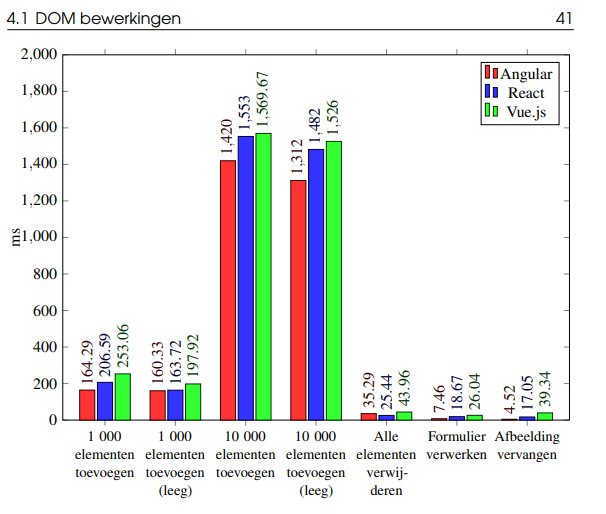
\includegraphics[width=0.7\textwidth]{Screenshot 2024-03-19 151509.png}
    \caption{Performantie van verschillende frameworks}
    \label{fig:Performantie}
\end{figure}

\begin{figure}[h]
    \centering
    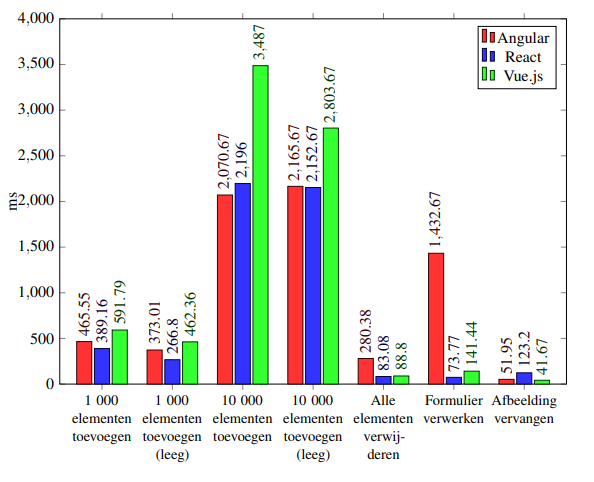
\includegraphics[width=0.7\textwidth]{Screenshot 2024-03-19 152515.png}
    \caption{Performantie van verschillende frameworks in android}
    \label{fig:PerformantieAndroid}
\end{figure}

